% 2-15-rb-tree.tex

%%%%%%%%%%%%%%%%%%%%
\documentclass[a4paper, justified]{tufte-handout}

\input{hw-preamble} % feel free to modify this file
%%%%%%%%%%%%%%%%%%%%
\title{第4-3讲: 群同态基本定理与正规子群}
\me{朱宇博 }{191220186 }{}{}
\date{\zhtoday} % or like 2019年9月13日
%%%%%%%%%%%%%%%%%%%%
\begin{document}
\maketitle
%%%%%%%%%%%%%%%%%%%%
\noplagiarism % always keep this line
%%%%%%%%%%%%%%%%%%%%
\begin{abstract}
  % \begin{center}{\fcolorbox{blue}{yellow!60}{\parbox{0.65\textwidth}{\large 
  %   \begin{itemize}
  %     \item 
  %   \end{itemize}}}}
  % \end{center}
\end{abstract}
%%%%%%%%%%%%%%%%%%%%
\beginrequired

%%%%%%%%%%%%%%%
\begin{problem}[TJ 9-11]
Find five non-isomorphic groups of order 8.
\end{problem}

\begin{solution}
$\mathbb{Z}_2\times \mathbb{Z}_4$, $\mathbb{Z}_2\times\mathbb{Z}_2\times\mathbb{Z}_2$, $\mathbb{Z}_8$, $Q_8$, $D_4$
\end{solution}
%%%%%%%%%%%%%%%

%%%%%%%%%%%%%%%
\begin{problem}[TJ 9-16]
Find the order of each of the following elements.\\
(a) (3,4) in $\mathbb{Z}_4 \times \mathbb{Z}_6$\\
(b) (6,15,4) in $\mathbb{Z}_{30} \times \mathbb{Z}_{45}  \times \mathbb{Z}_{24}$\\
(c) (5,10,15) in $\mathbb{Z}_{25} \times \mathbb{Z}_{25}  \times \mathbb{Z}_{25}$ \\
(d) (8,8,8) in $\mathbb{Z}_{10} \times \mathbb{Z}_{24}  \times \mathbb{Z}_{80}$

\end{problem}

\begin{solution}
(a)\\
3在$\mathbb{Z}_4$中的order是4,4在$\mathbb{Z}_6$中的order是3,故(3,4)的order为lcm(3,4)=12\\
(b)\\
6在$\mathbb{Z}_{30}$中的order是5,15在$\mathbb{Z}_{45}$中的order是3,4在$\mathbb{Z}_{24}$中的order是6,故(3,5,6)的order为lcm(3,5,6)=30\\
(c)\\
5在$\mathbb{Z}_{25}$中的order是5,10在$\mathbb{Z}_{25}$中的order是5,15在$\mathbb{Z}_{25}$中的order是5,故(5,10,15)的order为lcm(5,10,15)=5\\
(d)\\
8在$\mathbb{Z}_{10}$中的order是5,8在$\mathbb{Z}_{24}$中的order是3,8在$\mathbb{Z}_{80}$中的order是10,故(8,8,8)的order为lcm(5,3,10)=30\\
\end{solution}
%%%%%%%%%%%%%%%

%%%%%%%%%%%%%%%
\begin{problem}[TJ 9-23]
Prove or disprove the following assertion. Let $G$, $H$, and $K$ be groups. If $G \times K \cong H  \times K$, then $G \cong H$.
\end{problem}

\begin{solution}
True.\\
$G \times K \cong H  \times K$, 可知存在一个双射$\sigma: G\times K \to H\times K$, 且满足
\[
\sigma((g_1\circ g_2,k_1 \circ k_2))=\sigma((g_1,k_1))\circ\sigma((g_2,k_2))
\]
设函数$\phi: H\times K \to H : \phi(h,k)=h, h\in H,k\in K$\\
现证引理:对于任意的$k\in K$ ,对于固定的$g_1\in G$,存在唯一的$h_1\in H$, 使得$\phi(\sigma((g_1, k)))=h_1$\\
反证法: 假设存在$k_1,k_2$,使得$\phi(\sigma((g_1, k_1)))\neq \phi(\sigma((g_1, k_2)))$\\
则存在$g_2$, 使得
\[
\sigma((g_1,k_1))\circ\sigma((g_2, k))=\sigma((g_1\circ g_2,k_1\circ k))
\]
则有
\[
\phi(\sigma((g_1,k_1)))\circ\phi(\sigma((g_2, k)))=\phi(\sigma((g_1\circ g_2,k_1\circ k)))
\]
则对$(g_1,k_2)$有
\[
\phi(\sigma((g_1,k_2)))\circ\phi(\sigma((g_2, k)))\neq \phi(\sigma((g_1\circ g_2,k_2\circ k)))
\]
与同构定义相矛盾,故引理得证\\
定义函数$\sigma_2: G \to H, \sigma_2(g)=h$ 当且仅当存在$k_1,k_2$使得$\sigma(g,k_1)=(h,k_2)$\\
由引理易得函数2为双射函数。由函数$\sigma$的同构性质易得函数$\sigma_2$满足同构性质$\sigma_2(a)\circ\sigma_2(b)=\sigma_2(a\circ b)$\\
综上,有$G\cong H$
\end{solution}
%%%%%%%%%%%%%%%

%%%%%%%%%%%%%%%
\begin{problem}[TJ 10-1(a,c)]
For each of the following groups G, determine whether H is a normal subgroup of G. If H is a normal subgroup, write out a Cayley table for the factor group G/H.\\
(a)$G=S_4$ and $H=A_4$\\
(c)$G=S_4$ and $H=D_4$
\end{problem}

\begin{solution}
(a)\\
对于任意的$g \in A_4$, 则$g$为偶排列,$g^{-1}$为偶排列,则$gA_4g^{-1}$仍为偶排列,$gA_4g^{-1}\subset A_4$\\
对于任意的$g \in S_4/A_4$, 则$g$为奇排列,$g^{-1}$为奇排列,则$gA_4g^{-1}$为偶排列,$gA_4g^{-1}\subset A_4$\\
故$\forall g \in A_4, gA_4g^{-1}\subset A_4$\\
故$H$为$G$的Normal group.\\
对于$A_4$,其coset为$A_4, (12)A_4$\\
\begin{figure}[htbp]
    \centering
    \includegraphics[width = 0.30\linewidth]{figs/a}
  \end{figure}
 (b)\\
对于$g=(1,2)\in G, h = (1,2,3,4)\in H, ghg^{-1}=(1342)\notin H$\\
故$H$不为$G$的Normal group.\\
\end{solution}
%%%%%%%%%%%%%%%

%%%%%%%%%%%%%%%
\begin{problem}[TJ 10-11]
If a group G has exactly one subgroup H of order k, prove that H is normal in G.
\end{problem}

\begin{solution}
由Proposition 6.9可知,$|gH|=|H|$\\
由Theorem 6.8可知,$|gH|=|Hg|$\\
因为只有一个子群的order是k,故$gH=Hg$, $H$为normal group
\end{solution}
%%%%%%%%%%%%%%%


%%%%%%%%%%%%%%%
\begin{problem}[TJ 10-12]
Define the centralizer of an element g in a group G to be the set 
\[
C(g) = \{x \in G : xg = gx\}.
\]
Show that C(g) is a subgroup of G. If g generates a normal subgroup of G, prove that C(g) is normal in G.
\end{problem}

\begin{solution}
Prove: $C(g)$  is a subgroup of G\\
$eg=eg \to e \in C(g)$\\
$\forall h\in C(g), hg=gh\to g = h^{-1}gh\to gh^{-1}=h^{-1}g\to h^{-1}\in C(G)$\\
$\forall h_1,h_2\in C(g), (h_1g=gh_1, h_2g=gh_2)\to h_1h_2g = h_1gh_2=gh_1h_2\to h_1h_2\in C(g)$\\
综上,$C(g)$是$G$的subgroup.\\

\noindent Prove: If g generates a normal subgroup of G, prove that C(g) is normal in G.\\
引理1: $\forall x \in g, xg^{n}=g^{n}x$\\
Since $xg^{n}=gxg^{n-1}=g^2xg^{n-2}=...=g^nx$.\\

\noindent $\forall h\in G, hgh^{-1}=g^{n}\to \exists i,  hg^{i}h^{-1}=g$	
因此可将$h$写为$ghg^{-i}$\\
对于任意的$x\in C(G), hxh^{-1}=ghg^{-i}xg^{i}h^{-1}g^{-1}$。由引理1,我们可以得到$hxh^{-1}=ghg^{-i}xg^{i}h^{-1}g^{-1}=ghxh^{-1}g{-1}$。\\
可以得到$ghxh^{-1}=hxh^{-1}g$。因此$hxh^{-1}\in C(g)$。由定义可知,$C(G)$是normal group.
\end{solution}
%%%%%%%%%%%%%%%


%%%%%%%%%%%%%%%
\begin{problem}[TJ 11-5]
Describe all of the homomorphisms from $\mathbb{Z}_{24}$ to $\mathbb{Z}_{18}$.
\end{problem}
\begin{solution}
$\phi: \mathbb{Z}_{24}\to \mathbb{Z}_{18} : \phi(g)=kg \mod 18(k = 0, 3, 6, 9, 12, 15)$
\end{solution}
%%%%%%%%%%%%%%%

%%%%%%%%%%%%%%%
\begin{problem}[TJ 11-2(b,d,e)]
\end{problem}

\begin{solution}
(b)\\
 $$\begin{pmatrix}1&0\\
			   a&1\\
     \end{pmatrix}
     \begin{pmatrix}1&0\\
			   b&1\\
     \end{pmatrix}
     =
   \begin{pmatrix}1&0\\
			   a+b&1\\
     \end{pmatrix}$$\\
$\phi(a)\phi(b)=\phi(ab)$, 故为同态\\
kernel:\{0\}\\
(d)\\
$\phi(a)\phi(b)=\phi(ab)$, (行列式的性质)。故为同态\\
kernel:所有行列式等于$0$的二阶矩阵。\\
(e)\\
$\phi(a)\phi(b)=\phi(ab)$, 故为同态。\\
kernel:所有$b=0$的二阶矩阵。\\
\end{solution}
%%%%%%%%%%%%%%%


%%%%%%%%%%%%%%%%%%%%
\beginoptional

%%%%%%%%%%%%%%%

%%%%%%%%%%%%%%%
\begin{problem}[SageMath学习]
学习 TJ 第9、10/11章 关于 SageMath 的内容
\end{problem}

\begin{solution}
\end{solution}
%%%%%%%%%%%%%%%

%%%%%%%%%%%%%%%
\begin{problem}[TJ 11-17]
\end{problem}

\begin{solution}
\end{solution}
%%%%%%%%%%%%%%%


%%%%%%%%%%%%%%%
\begin{problem}[6、8阶群]
请给出同构意义下的所有6阶、8阶群。
\end{problem}

\begin{solution}
\end{solution}
%%%%%%%%%%%%%%%

%%%%%%%%%%%%%%%%%%%%
\beginot
%%%%%%%%%%%%%%%
\begin{ot}[群同态第二定理]
请证明群同态第二定理。
\end{ot}

% \begin{solution}
% \end{solution}
%%%%%%%%%%%%%%%

%%%%%%%%%%%%%%%

\begin{ot}[同构猜想]


\begin{minipage}{\linewidth}

\centering
\vspace{5cm}
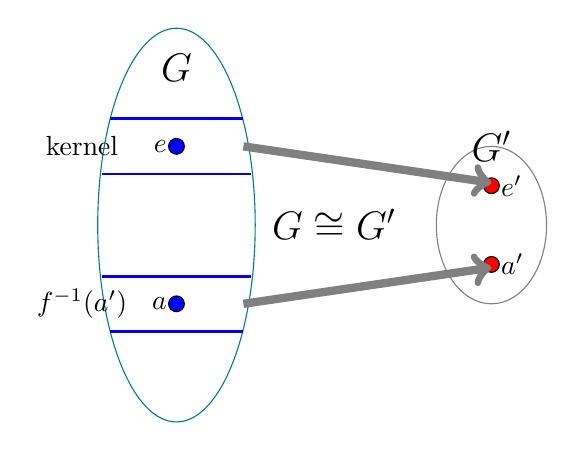
\begin{tikzpicture}

	\draw  (-2,1) [fill=blue]circle (0.1) node [left] {$e$};
	\draw  (-2,-1) [fill=blue]circle (0.1) node [left] {$a$};
	
	\draw (-2,0)[color=teal]circle (1 and 2.5);

	\draw   [ color=blue, line width=1pt] (-2.95,0.65)--(-1.05,0.65);
	\draw   [ color=blue, line width=1pt] (-2.85,1.35)--(-1.15,1.35);

	\draw   [ color=blue, line width=1pt] (-2.95,-0.65)--(-1.05,-0.65);
	\draw   [ color=blue, line width=1pt] (-2.85,-1.35)--(-1.15,-1.35);
		
	\draw  (2,0.5) [fill=red]circle (0.1) node (e1)[right]{$e'$};
	\draw  (2,-0.5) [fill=red]circle (0.1) node (a1)[right]{$a'$};
	
	\draw (2,0) [color= gray] circle (0.7 and 1);
	
	\draw [->,color=gray,line width=3pt,] (-1.15,1) to (e1);
	\draw [->,color=gray,line width=3pt,] (-1.15,-1) to (a1);
	
	\node at(-3.2,1){kernel};
	\node at (-3.2,-1){$f^{-1}(a')$};
	
	\node at (-2,2) {\Large \textbf{$G$}};
	
	\node at (2,1) {\Large \textbf{$G'$}};
	
	
	\node at (0,0) {\Large \textbf{$G\cong G'$}};
\end{tikzpicture}
\end{minipage}

请证明或证否下列猜想
\begin{itemize}
\item Kernel和任意的$G'$中非单位元元素的逆像不相交
\item Kernel和任意的$G'$中非单位元元素的逆像同势
\item 任意的$G'$中元素的逆像不相交且同势
\item 任意的$G'$中元素的逆像必定是kernel的某个陪集

\end{itemize}
\end{ot}


% \begin{solution}
% \end{solution}
%%%%%%%%%%%%%%%


% \vspace{0.50cm}
%%%%%%%%%%%%%%%
% \begin{ot}[]
% 
%   \noindent 参考资料:
%   \begin{itemize}
%     \item 
%   \end{itemize}
% \end{ot}

% \begin{solution}
% \end{solution}
%%%%%%%%%%%%%%%

%%%%%%%%%%%%%%%%%%%%
% 如果没有需要订正的题目,可以把这部分删掉

% \begincorrection
%%%%%%%%%%%%%%%%%%%%

%%%%%%%%%%%%%%%%%%%%
% 如果没有反馈,可以把这部分删掉
\beginfb

% 你可以写
% ~\footnote{优先推荐 \href{problemoverflow.top}{ProblemOverflow}}:
% \begin{itemize}
%   \item 对课程及教师的建议与意见
%   \item 教材中不理解的内容
%   \item 希望深入了解的内容
%   \item $\cdots$
% \end{itemize}
%%%%%%%%%%%%%%%%%%%%
% \bibliography{2-5-solving-recurrence}
% \bibliographystyle{plainnat}
%%%%%%%%%%%%%%%%%%%%
\end{document}